% !TeX root = ../report.tex
\section{Introduction to reinforcement learning}
Reinforcement learning is a machine learning paradigm dedicated to solving sequential decision processes. The definition of a reinforcement learning algorithm given by \citet[chap. 3]{RLBook2018}, is an algorithm which can solve a specific kind of sequential decision problem, namely those which can be described formally by a \textit{finite Markov decision process}.


\subsection{Finite Markov Decision Processes}

The Markov decision process provides a formal description of sequential decision problems. 

In this project, we define a Markov decision process by a 4-tuple $(\mathcal{S},\mathcal{A},\mathcal{R}, p)$, where $\mathcal{S}$ is the finite state-space, $\mathcal{A}$ is the finite action-space, $\mathcal{R} \subset \mathbb{R}$ is the finite reward-space, and the dynamics function $p : \mathcal{S} \times \mathcal{R} \times \mathcal{S} \times \mathcal{A} \rightarrow [0,1]$, defined in \cref{eq:p_def}, describes the conditional probability of entering a state $s' \in \mathcal{S}$ with reward $r \in \mathcal{R}$ given the previous state was $s \in \mathcal{S}$ and action $a \in \mathcal{A}(s)$ was chosen.
\begin{align}
    \label{eq:p_def} p(s',r\ |\ s,a) = \Pr{S_t\!=\!s', R_t\!=\!r\ |\ S_{t-1}\!=\!s, A_{t-1}\!=\!a}
\end{align}
Some like to include $\gamma$, a \textit{discount factor} in the definition of finite MDP. 
We, however, leave this definition to the individual reinforcement learning algorithm.


\vspace*{1em}

When solving Markov decision processes, a sequence of random variables is introduced. Let $T = \set{1, 2, \ldots}$ be a sequence of discrete time steps, $S_t$ is then a random variable which indicates the state of the environment at time step $t \in T$, $A_t$ is the action chosen at time step $t \in T$, from the set $\mathcal{A}(s)$ which denotes the actions available from state $s$. 
$R_t$ is the reward received after choosing action $A_{t-1}$ from state $S_{t-1}$

%\begin{align}
%    \sum_{s' \in \mycal{S}}\sum_{r \in \mycal{R}} p(s', r, s, a) &= 1 & \forall s \in \mycal{S}, \forall a \in \mycal{A}(s)\\
%    p(s'\ |\ s,a) \defeq \Pr{S_t=s'\ |\ S_{t-1} = s, A_{t-1} = a} &= \sum_{r\in \mycal{R}}p(s',r\ |\ s,a) & \forall s,s' \in \mycal{S}, \forall a \in \mycal{A}(s)\\
%    \Ex{R_t\ |\ S_{t-1}=s, A_{t-1}=a} &= \sum_{r \in \mycal{R}} r \sum_{s' \in \mycal{S}} p(s', r\ |\ s, a) & \forall s \in \mycal{S}, \forall a \in \mycal{A}(s)\\
%    \Ex{R_t\ |\ S_{t-1}=s, A_{t-1}=a, S_t=s'} &= \sum_{r \in \mycal{R}} r \frac{p(s', r\ |\ s, a)}{p(s'\ |\ s, a)} & \forall s,s' \in \mycal{S}, \forall a \in \mycal{A}(s)
%\end{align}
%\replace{Text for above}

\vspace*{1em}

\Cref{fig:agent-environment} visualises the agent-environment loop. 
Initially, the agent is placed in some environment \mycal{E}, from where the agent observes $S_0$.
The agent the chooses some action $A_0 \in \mycal{A}(S_0)$, after the action has been performed, state $S_{t+1}$ and $R_t$ is presented to the agent, this results in a sequence of the form $S_0,A_0,R_1,S_1,A_1,R_2,S_2,\ldots$

\begin{figure}[!htb]
    \centering
    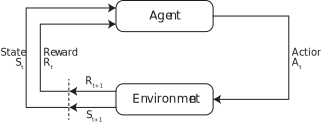
\includegraphics[scale=1]{../include/agent-environment-loop.pdf}
    \caption{The Agent-Environment interface adapted from \citet[chap. 3]{RLBook2018}}
    \label{fig:agent-environment}
\end{figure}

As such, the agent will learn the optimal \textit{policy} $\pi^*$ (or estimate thereof) by iteratively taking actions, and observing the following reward, and state of the environment.

To give a small example of the Markov decision process, consider the small grid world in \cref{fig:gridworld}. 
Suppose a robot is initially placed in square $a$, labeled \texttt{Start}, and that it has the goal of navigating to square $d$, labeled \texttt{End}. 
If the robot moves off the grid, it is returned to square $a$. 
Every move the robot makes have a cost of one, except for when successfully navigating to the \texttt{End} square, in which case it is rewarded with one point. 
Finally, suppose that the robot is faulty, and whenever it attempts to go right, there is a 20\% probability of moving diagonally down-right.
An MDP describing this problem is visualized in \cref{fig:gridworldMDP}.

\begin{figure}[!htb]
    \centering
    \begin{minipage}[t]{0.34\textwidth}
        \centering
        \raisebox{-0.5\height}{\hbox{\includegraphics{../include/PDF/gridworld2x2.pdf}}}
        \subcaption{2x2 gridworld}
        \label{fig:gridworld}
    \end{minipage}
    \begin{minipage}[t]{0.6\textwidth}
        \centering
        \raisebox{-0.5\height}{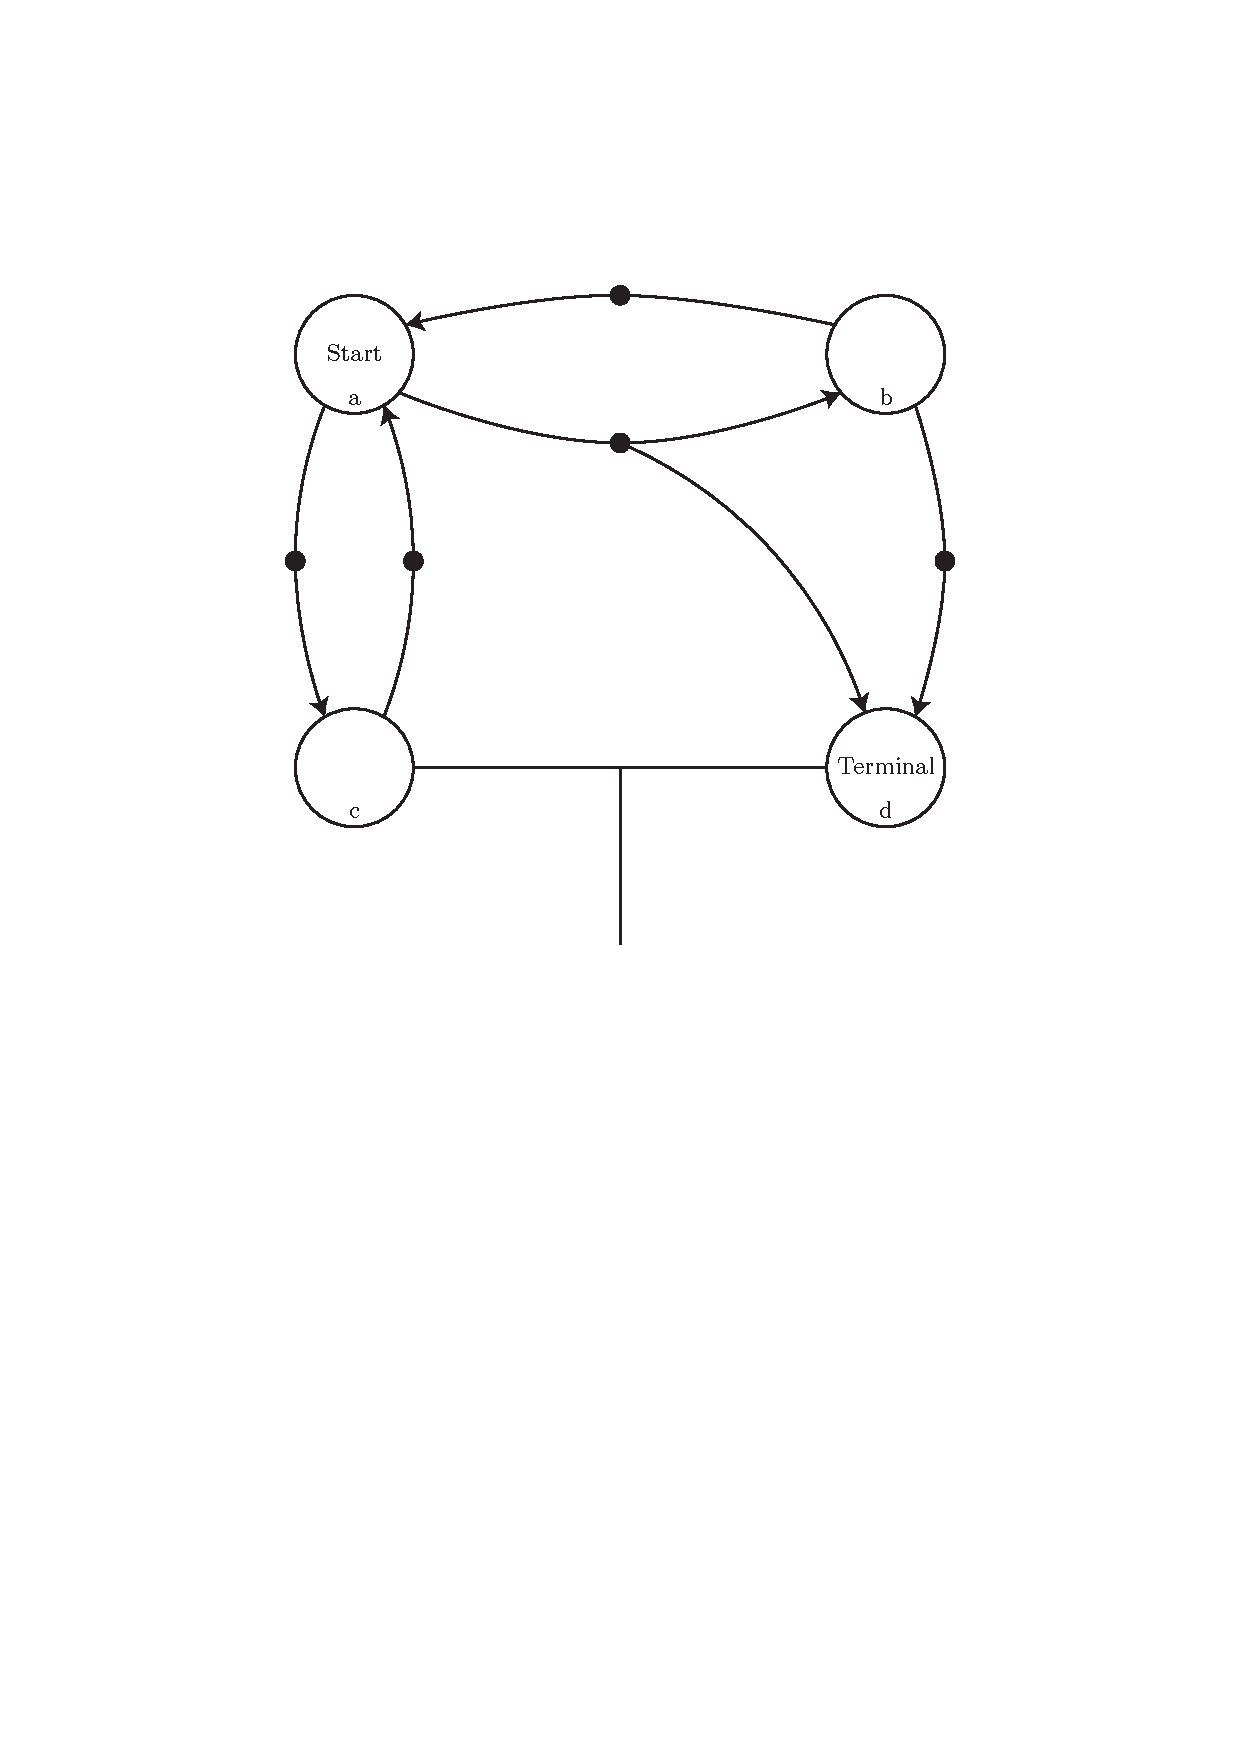
\includegraphics[scale=0.6]{../include/PDF/MDP.pdf}}
        \subcaption{MDP visualization of example gridworld with error prone right move}
        \label{fig:gridworldMDP}
    \end{minipage}
    \caption{Example environment (a) and MDP describing it (b)}
    \label{fig:MDP}
\end{figure}



\subsection{RL}



\subsubsection{Model-based \& Model-free}

\subsubsection{On-policy \& Off-policy}

\subsubsection{Reinforcement learning algorithm classes}
\paragraph{Action-Value}
\paragraph{Policy-Gradient}
\paragraph{Actor-Critic}

\subsubsection{Exploration vs Exploitation}
A great dilemma in the field of reinforcement learning is the choice of exploration vs. exploitation, when should the agent perform the action it deems best according to previous experience, and when should it explore new actions of which the outcome is less known? 
The most straightforward action-selection approach would be greedy action selection. With a greedy action selection, initial action values are essential, as otherwise, the agent may never explore some actions --- if there is an action which the agent has not yet attempted, it must see that action as attractive to get some idea of the usefulness of every action. 

An improvement to the greedy action selection, which has performed well historically is the $\epsilon-greedy$ approach, where the agent picks a random action with probability $\epsilon$, and a greedy action with probability $1-\epsilon$.

\begin{align}
    \Pr{A_t = a \in_R \mycal{A}(S_t)} &= \epsilon\\
    \Pr{A_t = \argmax_a \left[Q_t(S_t,a)\right]} &= 1-\epsilon
\end{align}

Where $Q_t$ is the action-value function estimate at time $t$.